%%%%%%%%%%%%%%%%%%%%%%%%%%%%%%%%%%%%%%%%%
% American Geophysical Union (AGU)
% LaTeX Template
% Version 1.0 (3/6/13)
%
% This template has been downloaded from:
% http://www.LaTeXTemplates.com
%
% Original author:
% The AGUTeX class and agu-ps referencing style were created and are owned 
% by AGU: http://publications.agu.org/author-resource-center/author-guide/latex-formatting-toolkit/
%
% This template has been modified from the blank AGU template to include
% examples of how to insert content and drastically change commenting. The
% structural integrity is maintained as in the original blank template.
%
% Important notes: 
% This template retains extensive commenting from the AGU template. It is heavily 
% advised you read these comments and follow them in order to insure a speedy 
% submission process.
%
%%%%%%%%%%%%%%%%%%%%%%%%%%%%%%%%%%%%%%%%%

%%%%%%%%%%%%%%%%%%%%%%%%%%%%%%%%%%%%%%%%%%%%%%%%%%%%%%%%%%%%%%%%%%%%%%%%%%%%
% AGUtmpl.tex: this template file is for articles formatted with LaTeX2e,
% Modified March 2013
%
% This template includes commands and instructions
% given in the order necessary to produce a final output that will
% satisfy AGU requirements.
%
% PLEASE DO NOT USE YOUR OWN MACROS
% DO NOT USE \newcommand, \renewcommand, or \def.
%
% FOR FIGURES, DO NOT USE \psfrag or \subfigure.
%
%%%%%%%%%%%%%%%%%%%%%%%%%%%%%%%%%%%%%%%%%%%%%%%%%%%%%%%%%%%%%%%%%%%%%%%%%%%%
%
% All questions should be e-mailed to latex@agu.org.
%
%%%%%%%%%%%%%%%%%%%%%%%%%%%%%%%%%%%%%%%%%%%%%%%%%%%%%%%%%%%%%%%%%%%%%%%%%%%%

% Step 1: Set the \documentclass

% There are two options for article format: two column (default) and draft.

% PLEASE USE THE DRAFT OPTION TO SUBMIT YOUR PAPERS.
% The draft option produces double spaced output.

% Choose the journal abbreviation for the journal you are submitting to:

% jgrga	JOURNAL OF GEOPHYSICAL RESEARCH
% gbc	GLOBAL BIOCHEMICAL CYCLES
% grl		GEOPHYSICAL RESEARCH LETTERS
% pal	PALEOCEANOGRAPHY
% ras	RADIO SCIENCE
% rog	REVIEWS OF GEOPHYSICS
% tec	TECTONICS
% wrr	WATER RESOURCES RESEARCH
% gc		GEOCHEMISTRY, GEOPHYSICS, GEOSYSTEMS
% sw	SPACE WEATHER
% ms	JAMES
%
%
%
% (If you are submitting to a journal other than jgrga,
% substitute the initials of the journal for "jgrga" below.)

\documentclass[draft,ms]{AGUTeX}

% cmz - Additional added packages
\usepackage{rotating}
\usepackage{color}

% To create numbered lines:

% If you don't already have lineno.sty, you can download it from http://www.ctan.org/tex-archive/macros/latex/contrib/ednotes/ (or search the internet for lineno.sty ctan), available at TeX Archive Network (CTAN). Take care that you always use the latest version.

% To activate the commands, uncomment \usepackage{lineno} and \linenumbers*[1]command, below:

\usepackage{lineno}
\linenumbers*[1]

%  To add line numbers to lines with equations:
%  \begin{linenomath*}
%  \begin{equation}
%  \end{equation}
%  \end{linenomath*}

%%%%%%%%%%%%%%%%%%%%%%%%%%%%%%%%%%%%%%%%%%%%%%%%%%%%%%%%%%%%%%%%%%%%%%%%%
% Figures and Tables

% DO NOT USE \psfrag or \subfigure commands.

%  Figures and tables should be placed AT THE END OF THE ARTICLE, after the references.

%  Uncomment the following command to include .eps files (comment out this line for draft format):
%\usepackage[dvips]{graphicx}
\usepackage{graphicx}

% Substitute one of the following for [dvips] above if you are using a different driver program and want to proof your illustrations on your machine:
% [xdvi], [dvipdf], [dvipsone], [dviwindo], [emtex], [dviwin],
% [pctexps],  [pctexwin],  [pctexhp],  [pctex32], [truetex], [tcidvi],
% [oztex], [textures]

%  Uncomment the following command to allow illustrations to print when using Draft:
\setkeys{Gin}{draft=false}

% Shortcuts (newcommands)
%% Remember to do a global replace on these before submission to AGU.
\newcommand{\degree}{$^{\circ}$}
\newcommand{\texttilde}{$\sim$}


% See how to enter figures and tables at the end of the article, after references.

%----------------------------------------------------------------------------------------
%	RUNNING HEAD AND CORRESPONDING AUTHOR
%----------------------------------------------------------------------------------------

% Author names in capital letters:
\authorrunninghead{SMITH ET AL.}

%------------------------------------------------

% Shorter version of title entered in capital letters:
\titlerunninghead{SHORT TITLE}

%------------------------------------------------

% Corresponding author mailing address and e-mail address:
\authoraddr{Corresponding author: Jane Smith, Department of Geography, Ohio State University, Columbus, Ohio, USA. (j.smith@ohio.edu)}

%----------------------------------------------------------------------------------------

\begin{document}

%----------------------------------------------------------------------------------------
%	TITLE
%----------------------------------------------------------------------------------------

\title{Title of the article}

%----------------------------------------------------------------------------------------
%	AUTHORS AND AFFILIATIONS
%----------------------------------------------------------------------------------------

% Use \author{\altaffilmark{}} and \altaffiltext{}

% \altaffilmark will produce footnote; matching \altaffiltext will appear at bottom of page.

\authors{Colin M. Zarzycki,\altaffilmark{1}
Kevin A. Reed,\altaffilmark{1}, and
Julio Bacmeister\altaffilmark{1}}

\altaffiltext{1}{Climate and Global Dynamics, National Center for Atmospheric Research, Boulder, Colorado, USA.}

%\altaffiltext{2}{Department of Geography, Ohio State University, Columbus, Ohio, USA.}

%----------------------------------------------------------------------------------------
%	ABSTRACT
%----------------------------------------------------------------------------------------

% Do NOT include any \begin...\end commands within the body of the abstract.

\begin{abstract}

The abstract goes here.

\end{abstract}

%----------------------------------------------------------------------------------------
%	ARTICLE CONTENT
%----------------------------------------------------------------------------------------

% The body of the article must start with a \begin{article} command
% \end{article} must follow the references section, before the figures and tables.

\begin{article}

\section{Introduction}

{\color{red}  Probably need a better introductory sentence or two.} The use of general circulation models (GCMs) to evaluate global tropical cyclone (TC) characteristics in current and future climate has grown considerably over the last decade.  It has been shown that GCMs can model TCs at horizontal resolutions upwards of 100 km with limitations \citep[e.g.,][]{Bengtsson2007a,Knutson2010,Strachan2013}. As GCMs have advanced to even higher horizontal resolutions ($\le 50$ km) the simulated climatology of tropical cyclones has improved greatly \citep[e.g.,][]{Oouchi2006,Zhao2009,Murakami2012,Manganello2012,Satoh2012,Bacmeister2014,Wehner2014,Reed2015}. Furthermore, the use of variable-resolution GCMs have shown to be useful for the study of regional TC climatologies at reduced computational cost compared to global high-resolution simulations \citep{Zarzycki2014AMIPTCs}.  

Recently, intercomparisons have shown that the range of simulated TC climatology across different climate models can be large \citep{Camargo2013CMIP,Walsh2015CLIVAR}.  It has also been shown that within individual GCMs TC characteristics can vary greatly depending on model design choices.  Numerous studies have documented the large uncertainty in TC simulations due to the choice of individual subgrid parameterizations, mainly cumulus parameterizations \citep[e.g.,][]{Kim2012,Reed2011CAMPhysics,Lim2014TCconv}), while others have focused on differences due to changes in whole parameterization suites \citep{Reed2011c,Bacmeister2014}. The dynamical core, the main fluid flow component of a GCM, has also been shown to be an important source of uncertainty for TC simulations, though less widely documented \citep{ReedSimplePhys,Zhao2012,Reed2015}.

In this manuscript we describe another mechanism through which simulated TC properties are influenced by model design choices, in particular, the manner in which the ocean and atmosphere are coupled within the climate system. Section \ref{sec:model} provides an introduction to the modeling system used in this study and how coupling between the atmosphere and ocean is treated. Section \ref{sec:forecast} details the sensitivity of TCs to the ocean grid using a deterministic forecast framework while Section \ref{sec:climate} investigates the impact on multi-year climate simulations. Section \ref{sec:discussion} assesses the results and offers further insight into their implications.

%------------------------------------------------

\section{Model description}
\label{sec:model}

\subsection{Community Atmosphere Model}
\label{subsec:cam}

In this paper, we utilize the Community Atmosphere Model (CAM), version 5 \citep{CAM5Tech}. The Spectral Element (SE) dynamical core option in CAM is used for all simulations. SE is the newest dynamical core available in CAM and is based upon continuous Galerkin spectral finite elements which are applied on a cubed-sphere grid \citep{Taylor1997,Thomas2005,Taylor2010,Dennis2012}. 

%CAM-SE has been shown to locally conserve both mass and tracer mass to machine precision, as well as moist total energy to the level of time truncation error in the absence of dissipative processes \citep{Taylor2011}. Additionally, since atmospheric primitive equations are solved locally on individual elements, interprocessor communication relative to more traditional atmospheric numerical schemes, giving CAM-SE attractive scaling properties \citep{Dennis2012,Evans2013}.

CAM-SE is coupled to land, ocean, and ice model components within the Community Earth System Modelling (CESM) framework. The land model is the Community Land Model (CLM) version 4.0 run in satellite phenology (SP) mode on a 0.23 by 0.31$^{\circ}$ latitude-longitude grid \citep{CLM40Tech}. While CESM also allows for coupling to dynamic ocean and ice models, all of the simulations in this project utilize prescribed SSTs and ice cover concentrations.

\subsection{Coupling within CESM}
\label{subsec:coupling}

Because earth system model components generally are not integrated on the same spatial grid, CPL7 is used to couple various systems within the CESM framework \citep{Craig2012}. The coupler utilizes conservative remapping weights to regrid quantities between model components.

{\color{red} (Describe coupling procedure in CESM; draw schematic; confirm with T. Craig or Mariana).}

During coupling between the atmosphere and ocean, state variables from the atmospheric grid are conservatively remapped to the ocean grid. Surface momentum stress ($\tau$) and sensible and latent heat fluxes are calculated on the ocean grid. The quantities are then passed back to the atmospheric grid, allowing these quantities to be available to both the atmospheric dynamical core and subgrid physical parameterizations.

Generally, if the atmosphere and ocean are not on the same grid, the atmospheric grid consists of finer grid spacing. 

Prescribed SSTs and ice are passed to the model on a 1\degree{}x1\degree{} grid and internally interpolated to the ocean and ice grids.

\section{Deterministic simulations}
\label{sec:forecast}

To assess the differences in simulated TCs in a controlled, deterministic manner, we utilize two nearly identical CAM setups to complete short-term forecast simulations of observed storms. These simulations utilize the new, variable-resolution capability of CAM-SE \citep{Zarzycki2014APE}.

The model is configured with an atmospheric grid with 1/8\degree{} (\texttilde{}14km) resolution over the Atlantic Ocean and are initialized with a digitally-filtered atmospheric analysis from the National Center for Atmospheric Predictions's Global Data Assimilation System (GDAS). Observed SSTs are taken from NOAAOI and provided as input to the model on a 1\degree{}x1\degree{} grid. The land surface is modeled by the Community Land Model (CLM) version 4.0 and is initialized with a state nudged to be in balance with the atmospheric initial conditions. The model setup and initialization are further detailed in \citet{Zarzycki2015TCForecast}.

The only difference between the two setups is the grid used by the data ocean and ice models. The first set of simulations uses a displaced tripole grid with an equivalent resolution of 1\degree{} (gx1v6) while the second uses an ocean grid identical to the atmospheric grid with an equivalent resolution of 1/8\degree{}. Since the SST and ice cover data are provided at coarser scales than the model interpolates to, any differences in the results arise due to the differences in calculating of surface fluxes and momentum drag on the corresponding ocean grids.

Figure \ref{fig:forecast_panels} shows the 120-hour forecast for Hurricane Leslie in the North Atlantic Ocean from the 2012 hurricane season. The simulation was initialized at 00Z on August 31st, 2012 and is valid at 00Z on September 5th, 2012. The forecast using the 1\degree{} ocean grid is on the left (Fig. \ref{fig:forecast_panels}a,c), with the 1/8\degree{} ocean grid on the right (Fig. \ref{fig:forecast_panels}b,d). All fields are extracted from the atmospheric model component. The top panels depict instantaneous lowest model level wind (black vectors) as well as the surface frictional stress vector (red). In the Fig. \ref{fig:forecast_panels}a, we note many instances where the vectors are not aligned. This results from the surface stress being calculated on the coarser grid. The atmospheric dynamical core then subsamples this coarser information to provide stress information at the same resolution used by the numerics. In Fig. \ref{fig:forecast_panels}b, the wind and stress vectors are essentially parallel (180\degree{} difference), indicating that the frictional drag is acting in parallel opposition to the wind. The higher resolution ocean grid preserves the resolution of the surface wind field during stress calculations. Additionally, the maximum magnitudes of the stress vectors are larger at the storm's radius of maximum wind in Fig. \ref{fig:forecast_panels}b. Since stress is directly correlated with the surface wind speed, this highlights that maxima in the wind field at the atmospheric grid cell scale are preserved with the higher resolution ocean grid, whereas these maxima are ``smoothed'' in the calculation where wind is first averaged to the coarser ocean grid (Fig. \ref{fig:forecast_panels}a). This is further evidenced by the fact that the integrated dot product (over a 5\degree{}x5\degree{} domain centered over the TC minimum surface pressure) of the two fields is approximately 10\% smaller in the simulations using the 1\degree{} ocean grid. Therefore, the use of the coarser ocean grid results in a weaker frictional force used by the atmospheric dynamics.

The cumulative surface heat flux is shown on the bottom (sensible plus latent) for the two storms at the same forecast time. It is readily apparent that the coarser ocean grid (Fig. \ref{fig:forecast_panels}c) provides information back to the atmosphere with significantly less spatial structure than the 1/8\degree{} ocean grid (Fig. \ref{fig:forecast_panels}d). While the difference in 5\degree{}x5\degree{} integrated heat flux is relatively small (approximately 1\%), it is clear that the spatial structure of the heat flux field is very different between the two model configurations. This may also play a role in storm dynamics with the 1\degree{} ocean grid providing a larger, more diffuse source of surface heating to the TC core than the high-resolution grid.

\subsection{Climate simulations}
\label{sec:climate}

{\color{red} JULIO/KEVIN CLIMATE SIMS}

%------------------------------------------------

\section{Discussion}
\label{sec:discussion}

{\color{red} Discussion goes here.}

The issues outlined in the manuscript are rather trivial to correct for data ocean models, where specifying SSTs and applying coupled atmosphere-ocean calculations on the same grid is straightforward. More problematic adjustments arise when coupling to a dynamical ocean model. The vast majority of coupled simulations not only utilize differing resolutions between different model components, but also different numerical techniques and grids. Therefore, remapping between components is an absolute necessity.

The obvious recommendation to alleviate coupling inconsistencies when it is not feasible to use identical grids is to calculate these quantities on the finest resolution grid of the coupled system. In the vast majority of earth system models, this is typically the atmosphere. Performing coupling in this manner ensures that information passed back to a model component has not be interpolated to a resolution coarser than the compnent's native resolution during the coupling process.

However, it is not clear that technique is fully appropriate for dynamical ocean models, where aspects such as turbulent mixing may be sufficiently non-linear that merely averaging from a higher resolution grid may not be the most appropriate mechanism.

%----------------------------------------------------------------------------------------
%	APPENDICES (OPTIONAL)
%----------------------------------------------------------------------------------------

%%%%%%%%%%%%%%%%%%%%%%%%%%%%%%%%
%% Optional Appendix goes here

% \appendix resets counters and redefines section heads
% but doesn't print anything.
% After typing  \appendix

% \section{Here Is Appendix Title}
% will show
% Appendix A: Here Is Appendix Title

%\appendix
%
%\section{Appendix Title}
%
%Vivamus magna enim, aliquet id cursus a, pharetra ut purus. Phasellus suscipit nisi iaculis mi vulputate id interdum velit dictum. Nam ullamcorper elit in lectus ultrices vitae volutpat massa gravida. Etiam sagittis commodo neque eget placerat. Sed et nisi faucibus metus interdum adipiscing id nec lacus. Donec ipsum diam, malesuada at euismod consectetur, placerat quis diam. Phasellus cursus semper viverra. Proin magna tortor, blandit in ultricies id, facilisis at nibh. Proin eu neque est. Etiam euismod auctor ante. Mauris mauris sem, tincidunt a placerat rutrum, porta id est. Aenean non velit porta eros condimentum facilisis at in nibh. Etiam cursus purus ut orci rhoncus sit amet semper eros porttitor. Etiam ac leo at ipsum tincidunt consequat ac non sapien. Aenean sed leo diam, venenatis pharetra odio.

%----------------------------------------------------------------------------------------
%	GLOSSARY OR NOTATION (OPTIONAL)
%----------------------------------------------------------------------------------------

%%%%%%%%%%%%%%%%%%%%%%%%%%%%%%%%%%%%%%%%%%%%%%%%%%%%%%%%%%%%%%%%
%
% Optional Glossary or Notation section, goes here
%
%%%%%%%%%%%%%%
% Glossary is only allowed in Reviews of Geophysics
% \section*{Glossary}
% \paragraph{Term}
% Term Definition here
%
%%%%%%%%%%%%%%
% Notation -- End each entry with a period.
% \begin{notation}
% Term & definition.\\
% Second term & second definition.\\
% \end{notation}
%%%%%%%%%%%%%%%%%%%%%%%%%%%%%%%%%%%%%%%%%%%%%%%%%%%%%%%%%%%%%%%%

%----------------------------------------------------------------------------------------
%	ACKNOWLEDGEMENTS
%----------------------------------------------------------------------------------------

\begin{acknowledgments}
This work was partially supported by a grant from the Spanish Ministry of Science and Technology.
\end{acknowledgments}

%----------------------------------------------------------------------------------------
%	BIBLIOGRAPHY
%----------------------------------------------------------------------------------------

% Either type in your references using
% \begin{thebibliography}{}
% \bibitem{}
% Text
% \end{thebibliography}

% Or,

% If you use BiBTeX for your references, please use the agufull08.bst file (available at % ftp://ftp.agu.org/journals/latex/journals/Manuscript-Preparation/) to produce your .bbl
% file and copy the contents into your paper here.

% Follow these steps:
% 1. Run LaTeX on your LaTeX file.

% 2. Make sure the bibliography style appears as \bibliographystyle{agufull08}. Run BiBTeX on your LaTeX
% file.

% 3. Open the new .bbl file containing the reference list and
%   copy all the contents into your LaTeX file here.

% 4. Comment out the old \bibliographystyle and \bibliography commands.

% 5. Run LaTeX on your new file before submitting.

% AGU does not want a .bib or a .bbl file. Please copy in the contents of your .bbl file here.

%\begin{thebibliography}{}
\bibliographystyle{agufull08}
\bibliography{references}
%\end{thebibliography}

%\begin{thebibliography}{}
%
%\providecommand{\natexlab}[1]{#1}
%\expandafter\ifx\csname urlstyle\endcsname\relax
%  \providecommand{\doi}[1]{doi:\discretionary{}{}{}#1}\else
%  \providecommand{\doi}{doi:\discretionary{}{}{}\begingroup
%  \urlstyle{rm}\Url}\fi
%
%\bibitem[{\textit{Atkinson and Sloan}(1991)}]{AtkinsonSloan}
%Atkinson, K., and I.~Sloan (1991), The numerical solution of first-kind
%  logarithmic-kernel integral equations on smooth open arcs, \textit{Math.
%  Comp.}, \textit{56}(193), 119--139.
%
%\end{thebibliography}

% Reference citation examples:

%...as shown by \textit{Kilby} [2008].
%...as shown by {\textit  {Lewin}} [1976], {\textit  {Carson}} [1986], {\textit  {Bartholdy and Billi}} [2002], and {\textit  {Rinaldi}} [2003].
%...has been shown [\textit{Kilby et al.}, 2008].
%...has been shown [{\textit  {Lewin}}, 1976; {\textit  {Carson}}, 1986; {\textit  {Bartholdy and Billi}}, 2002; {\textit  {Rinaldi}}, 2003].
%...has been shown [e.g., {\textit  {Lewin}}, 1976; {\textit  {Carson}}, 1986; {\textit  {Bartholdy and Billi}}, 2002; {\textit  {Rinaldi}}, 2003].

%...as shown by \citet{jskilby}.
%...as shown by \citet{lewin76}, \citet{carson86}, \citet{bartoldy02}, and \citet{rinaldi03}.
%...has been shown \citep{jskilbye}.
%...has been shown \citep{lewin76,carson86,bartoldy02,rinaldi03}.
%...has been shown \citep [e.g.,][]{lewin76,carson86,bartoldy02,rinaldi03}.

% Please use ONLY \citet and \citep for reference citations.
% DO NOT use other cite commands (e.g., \cite, \citeyear, \nocite, \citealp, etc.).

\end{article}

%----------------------------------------------------------------------------------------
%	FIGURES AND TABLES
%----------------------------------------------------------------------------------------

%% Enter Figures and Tables here:
%
% DO NOT USE \psfrag or \subfigure commands.
%
% Figure captions go below the figure.
% Table titles go above tables; all other caption information should be placed in footnotes below the table.
%
%----------------
% EXAMPLE FIGURE
%
% \begin{figure}
% \noindent\includegraphics[width=20pc]{samplefigure.eps}
% \caption{Caption text here}
% \label{figure_label}
% \end{figure}
%
% ---------------
% EXAMPLE TABLE
%
%\begin{table}
%\caption{Time of the Transition Between Phase 1 and Phase 2\tablenotemark{a}}
%\centering
%\begin{tabular}{l c}
%\hline
% Run  & Time (min)  \\
%\hline
%  $l1$  & 260   \\
%  $l2$  & 300   \\
%  $l3$  & 340   \\
%  $h1$  & 270   \\
%  $h2$  & 250   \\
%  $h3$  & 380   \\
%  $r1$  & 370   \\
%  $r2$  & 390   \\
%\hline
%\end{tabular}
%\tablenotetext{a}{Footnote text here.}
%\end{table}

% See below for how to make sideways figures or tables.

\newpage

\begin{figure}
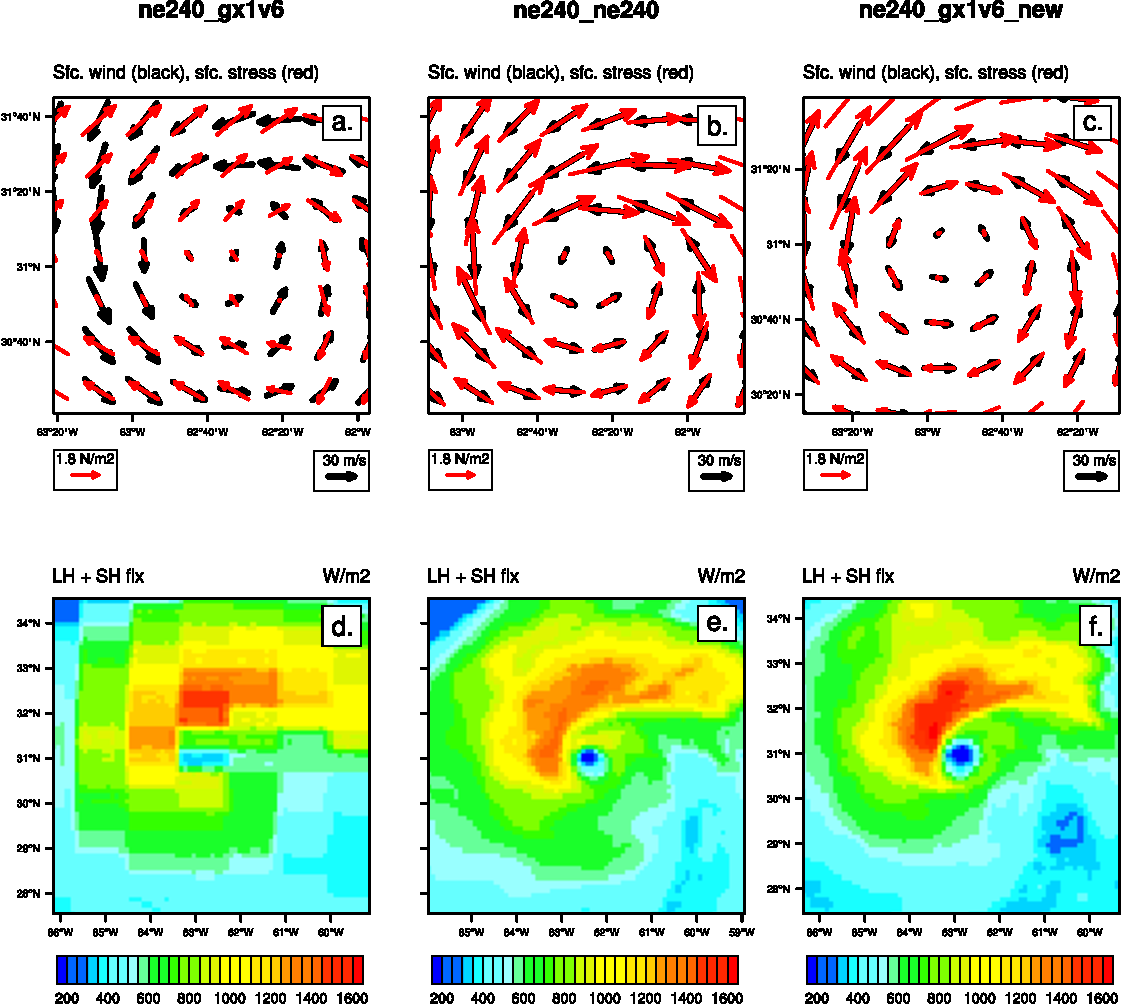
\includegraphics[width=0.8\linewidth]{fig_compareStress.pdf}
\caption{Figure caption}
\label{fig:forecast_panels}
\end{figure}

%\begin{table}
%\caption{Table caption}\label{sampletable}
%\begin{tabular}{l l l}
%\hline
%\textbf{Treatments} & \textbf{Response 1} & \textbf{Response 2}\\
%\hline
%Treatment 1 & 0.0003262 & 0.562 \\
%Treatment 2 & 0.0015681 & 0.910 \\
%Treatment 3 & 0.0009271 & 0.296 \\
%\hline
%\end{tabular}
%\end{table}

\end{document}

%%%%%%%%%%%%%%%%%%%%%%%%%%%%%%%%%%%%%%%%%%%%%%%%%%%%%%%%%%%%%%%

More Information and Advice:

%% ------------------------------------------------------------------------ %%
%
%  SECTION HEADS
%
%% ------------------------------------------------------------------------ %%

% Capitalize the first letter of each word (except for
% prepositions, conjunctions, and articles that are
% three or fewer letters).

% AGU follows standard outline style; therefore, there cannot be a section 1 without
% a section 2, or a section 2.3.1 without a section 2.3.2.
% Please make sure your section numbers are balanced.
% ---------------
% Level 1 head
%
% Use the \section{} command to identify level 1 heads;
% type the appropriate head wording between the curly
% brackets, as shown below.
%
%An example:
%\section{Level 1 Head: Introduction}
%
% ---------------
% Level 2 head
%
% Use the \subsection{} command to identify level 2 heads.
%An example:
%\subsection{Level 2 Head}
%
% ---------------
% Level 3 head
%
% Use the \subsubsection{} command to identify level 3 heads
%An example:
%\subsubsection{Level 3 Head}
%
%---------------
% Level 4 head
%
% Use the \subsubsubsection{} command to identify level 3 heads
% An example:
%\subsubsubsection{Level 4 Head} An example.
%
%% ------------------------------------------------------------------------ %%
%
%  IN-TEXT LISTS
%
%% ------------------------------------------------------------------------ %%
%
% Do not use bulleted lists; enumerated lists are okay.
% \begin{enumerate}
% \item
% \item
% \item
% \end{enumerate}
%
%% ------------------------------------------------------------------------ %%
%
%  EQUATIONS
%
%% ------------------------------------------------------------------------ %%

% Single-line equations are centered.
% Equation arrays will appear left-aligned.

Math coded inside display math mode \[ ...\]
 will not be numbered, e.g.,:
 \[ x^2=y^2 + z^2\]

 Math coded inside \begin{equation} and \end{equation} will
 be automatically numbered, e.g.,:
 \begin{equation}
 x^2=y^2 + z^2
 \end{equation}

% IF YOU HAVE MULTI-LINE EQUATIONS, PLEASE
% BREAK THE EQUATIONS INTO TWO OR MORE LINES
% OF SINGLE COLUMN WIDTH (20 pc, 8.3 cm)
% using double backslashes (\\).

% To create multiline equations, use the
% \begin{eqnarray} and \end{eqnarray} environment
% as demonstrated below.
\begin{eqnarray}
  x_{1} & = & (x - x_{0}) \cos \Theta \nonumber \\
        && + (y - y_{0}) \sin \Theta  \nonumber \\
  y_{1} & = & -(x - x_{0}) \sin \Theta \nonumber \\
        && + (y - y_{0}) \cos \Theta.
\end{eqnarray}

%If you don't want an equation number, use the star form:
%\begin{eqnarray*}...\end{eqnarray*}

% Break each line at a sign of operation
% (+, -, etc.) if possible, with the sign of operation
% on the new line.

% Indent second and subsequent lines to align with the first character following the equal sign on the first line.

% Use an \hspace{} command to insert horizontal space into your equation if necessary. Place an appropriate unit of measure between the curly braces, e.g. \hspace{1in}; you may have to experiment to achieve the correct amount of space.


%% ------------------------------------------------------------------------ %%
%
%  EQUATION NUMBERING: COUNTER
%
%% ------------------------------------------------------------------------ %%

% You may change equation numbering by resetting
% the equation counter or by explicitly numbering
% an equation.

% To explicitly number an equation, type \eqnum{}
% (with the desired number between the brackets)
% after the \begin{equation} or \begin{eqnarray}
% command.  The \eqnum{} command will affect only
% the equation it appears with; LaTeX will number
% any equations appearing later in the manuscript
% according to the equation counter.
%

% If you have a multiline equation that needs only
% one equation number, use a \nonumber command in
% front of the double backslashes (\\) as shown in
% the multiline equation above.

%% ------------------------------------------------------------------------ %%
%
%  SIDEWAYS FIGURE AND TABLE EXAMPLES
%
%% ------------------------------------------------------------------------ %%
%
% For tables and figures, add \usepackage{rotating} to the paper and add the rotating.sty file to the folder.
% AGU prefers the use of {sidewaystable} over {landscapetable} as it causes fewer problems.
%
% \begin{sidewaysfigure}
% \includegraphics[width=20pc]{samplefigure.eps}
% \caption{caption here}
% \label{label_here}
% \end{sidewaysfigure}
%
% \begin{sidewaystable}
% \caption{}
% \begin{tabular}
% Table layout here.
% \end{tabular}
% \end{sidewaystable}